%%%%%%%%%%%%%%%%%%%%%%%%%%%%%%%%%%%%%%%%%%%%%%%%%%%%%%%%%%%
%% Flujo de trabajo

\section{Flujo de trabajo y control de versiones}\label{flujo:flujo-de-trabajo}

\subsection{Metodología Kanban}\label{flujo:metodologia-kanban}
\subsubsection{El Tablero Kanban}\label{flujo:tablero-kanban}
Trello será la herramienta principal para mantener la coordinación del flujo de trabajo a través de un \textbf{Tablero Kanban}. Para el desarrollo del proyecto dividiremos el trabajo en tareas y las iremos incorporando a este tablero dentro de columnas que vienen a representar nuestros procesos de producción.

La idea es anotar cada tarea del proyecto en una tarjeta y agregarla a la columna de la izquierda. Mientras se trabaja en la tarea, su tarjeta va avanzando de izquierda a derecha hasta llegar a la última columna.  

\begin{figure}[h]
	\centering
	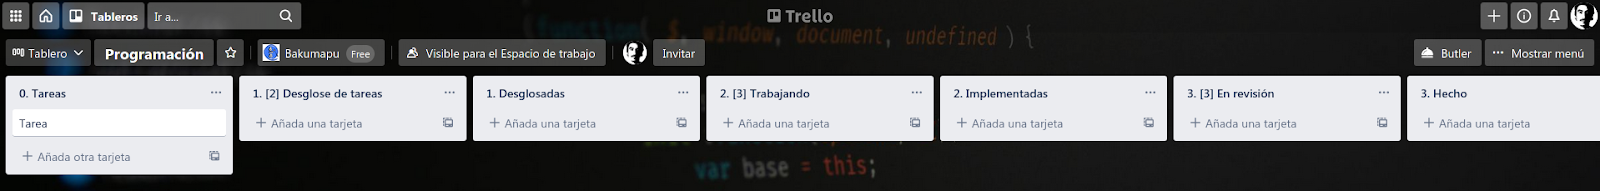
\includegraphics[width=\textwidth]{imágenes/tablero01.png}
	\caption{Tablero Kanban en Trello.}
\end{figure}

\subsubsection{Límites de trabajo y columnas asociadas}\label{flujo:limites-de-trabajo}
Cada columna tiene asociado un límite máximo de tareas simultáneas (\lsc{WIP}) por lo que si el límite ha sido alcanzado no se podrán incorporar nuevas tareas a la columna hasta haber avanzado una de sus tarjetas a la columna siguiente. Este límite se puede ver en el número dentro de llaves [~].

Al mismo tiempo, cada columna tendrá una división vertical, dejando a la izquierda las tareas en proceso y a la derecha las tareas que ya han completado la etapa. El límite es compartido por ambas secciones, por lo que independiente de la sección en la que se encuentre la tarjeta, no puede haber más tarjetas que el límite establecido en la columna.

Lamentablemente la plataforma Trello no permite dividir una misma columna en dos secciones, por lo que se añadirá una enumeración al nombre de cada columna que se repetirá en los casos de columnas asociadas. Por ejemplo en la \autoref{flujo:figura-wip}, sumando las tareas de la columna “2. [5] Trabajando” y las de la columna “2. Terminadas” solo puede haber 5 tareas simultáneas por lo que no deberemos añadir una sexta.

\begin{figure}[h]
	\centering
	\caption{Límites de trabajo en Trello.}
	\label{flujo:figura-wip}
	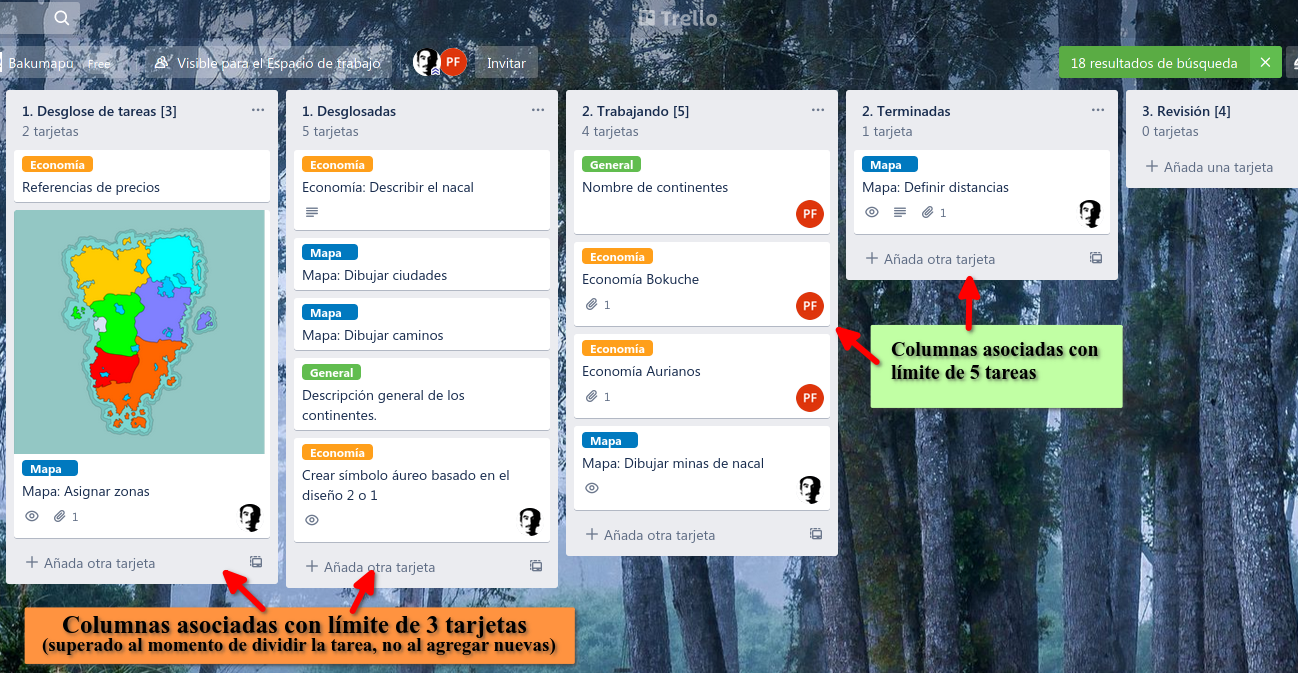
\includegraphics[width=\textwidth]{imágenes/tablero02.png}
\end{figure}

Respetar los límites de cada columna, facilitará la distribución de trabajo en un modelo de entrega continua y nos permitirá tomar decisiones más acertadas y realistas al momento de la planificación.

\subsubsection{Descripción de columnas}\label{flujo:descripcion-de-columnas}
El funcionamiento de cada columna es bastante sencillo:
\begin{enumerate}
	\item \textbf{Columna Tareas:} Acá dejamos las tareas en sus tarjetas y las ordenamos según prioridad (arriba más urgentes). Solo se debería empezar a trabajar en la tarea superior. La prioridad de las tareas será determinada por el equipo.
	\item \textbf{Columna Desglose de tareas:} Es \textit{muy importante} que las tareas sean descompuestas en tareas sencillas para que no se demoren más de unos días en completarse. Las tareas que entran a esta columna se analizan y dividen en tareas acotadas.
	\item \textbf{Columna Desglosadas:} Aquí las tareas desglosadas esperan hasta que alguien se haga cargo de implementar el código y pasan a la siguiente columna.
	\item \textbf{Columna Trabajando:} Aquí el encargado se anota en la tarjeta y trabaja hasta completarla, pasándola a Terminadas. Una tarea se considerará completada solo cuando haya pasado todos los test correspondientes.
	\item \textbf{Columna Implementadas:} Acá quedan las tarjetas con tareas terminadas esperando revisión.
	\item \textbf{Columna En revisión:} Acá van las tareas que se estén revisando. Si tienen problemas o bugs pequeños se resuelven aquí mismo, si tuviera bugs o un problema más grande podría volver a analizarse el desglose con alta prioridad.
	\item \textbf{Columna Hecho:} Aquí van las tareas terminadas. Se eliminan al hacer el merge de un conjunto de features completo a develop (cuando sube la versión).
\end{enumerate}

\subsubsection{Flexibilidad}\label{flujo:flexibilidad}
Esta es una herramienta que permite tener visualizadas las distintas áreas del proyecto, identificar cuellos de botella y contribuir a la gestión mediante límites de trabajo; no obstante, no debe olvidarse que es solo una guía. Si algo del sistema necesita cambiarse porque va contra el flujo de trabajo, se debe ajustar rápidamente.

\subsubsection{Nombres de Tarjetas}\label{flujo:nombres-de-tarjetas}
Los nombres de las tareas se deben corresponder con la tarea o funcionalidad a implementar y a su rama asociada en \lsc{GIT}. Más detalles en el apartado \nameref{organizacion:nombres-de-ramas}.

%%%%%%%%%%%%%%%%%%%%%%%%%%%%%%%%%%%%%%%%%%%%%%%%%%%%%%%%%%%
%%%%%%%%%%%%%%%%%%%%%%%%%%%%%%%%%%%%%%%%%%%%%%%%%%%%%%%%%%%

%\pagebreak
\subsection{Repositorio}\label{flujo:repositorio}
El repositorio \lsc{GIT} de Bakumapu se encuentra alojado en la siguiente dirección: \url{https://github.com/polirritmico/Bakumapu}.

La contribución de código será organizada a través del modelo de ramas de función (feature branching) adaptada a un sistema de TDD de entrega continua (más información en el apartado \nameref{principios:principios-de-diseno}).

\subsubsection{Modelo de Ramas de función}\label{flujo:modelo-de-ramas}
\begin{figure}[H]
	\centering
	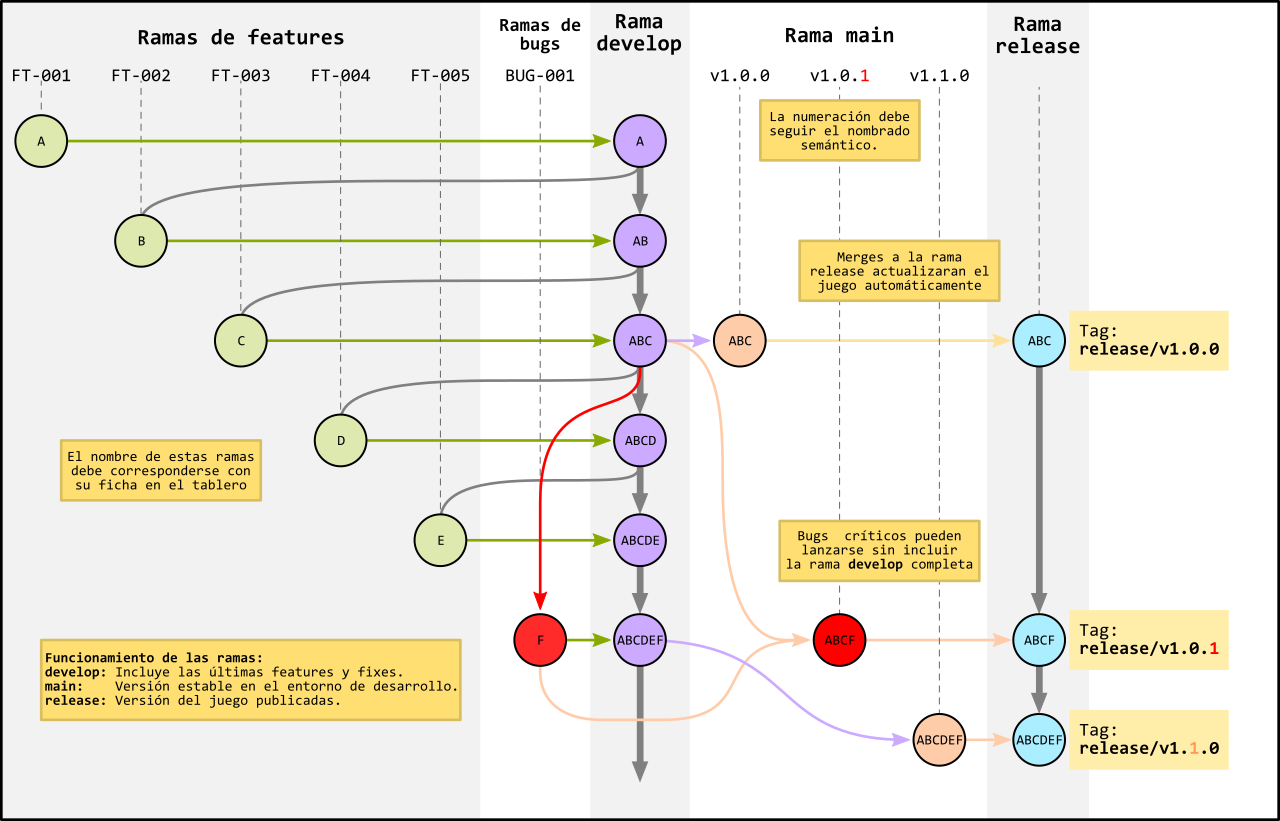
\includegraphics[width=\textwidth]{imágenes/git.png}
	\caption{Ramas en \lsc{GIT}.}
\end{figure}

\Needspace{3\baselineskip}
\noindent\textbf{Ramas principales.}\label{flujo:ramas-principales}

\noindent Bakumapu contará con 3 ramas principales, \textbf{develop}, \textbf{main} y \textbf{release}:

\begin{enumerate}
	\renewcommand{\labelenumi}{\alph{enumi}.}
	\item \textbf{develop:} Esta rama contará siempre con las últimas funciones implementadas. Es la rama principal del desarrollo ya que para trabajar cada feature, se creará una rama a partir de \textbf{develop}. A medida que se avance esa implementación continuamente se harán merges de vuelta a \textbf{develop} (al menos uno al día)\footnote{Es muy importante este punto porque el tiempo que el código de la rama permanezca fuera de develop puede generar bugs desconocidos al estar aislado de los commit de otras ramas.}. De esta forma se pretende que esté siempre disponible el código completo para no perder la referencia global del proyecto. 
	
	\item \textbf{main:} En esta rama se tratará de mantener el código lo más estable posible. Representa la última entrega del desarrollo y por lo tanto se creará a partir de \textbf{develop} cuando el código haya completado el conjunto de features de cada etapa de implementación del proyecto. Los testers trabajarán en base a esta rama. 
	
	\item \textbf{release:} Se creará a partir \textbf{main} una vez que esta haya sido extensamente probada y depurada. Esta rama será la que pasará el código a producción por eso debe ser la más robusta (por ejemplo deploys automáticos a todas las copias instaladas y conectadas a internet).
\end{enumerate}

\paragraph{Ramas de implementación}\label{pg:ramas-de-implementacion}
\begin{enumerate}
	\renewcommand{\labelenumi}{\alph{enumi}.}
	\item \textbf{Ramas de features:} Debe crearse una para cada funcionalidad que se quiera implementar a partir del estado actual de la rama \textbf{develop}. El nombre de la rama debe comenzar con “\textbf{ft-}” y corresponderse con el de su tarjeta asociada en el tablero (apartado \nameref{flujo:nombres-de-tarjetas}). La idea es desarrollar test que permitan verificar el funcionamiento de la feature y que deben ser superados antes de dar por concluido el trabajo en la rama. De esta forma se intentará hacer continuos merges hacia \textbf{develop} con la certeza de haber superado los test.
	
	\item \textbf{Ramas de bugs:} Debe crearse una por cada bug encontrado. Dependiendo del bug la rama será creada a partir de \textbf{main}, \textbf{develop} o \textbf{release}. El merge del fix deberá ser hacia \textbf{develop} y si corresponde también a \textbf{release}. El nombre de la rama debe comenzar con “\textbf{bug-}” y corresponderse con el de su tarjeta asociada en el tablero (apartado \nameref{organizacion:nombres-de-ramas}).
\end{enumerate}

\subsubsection{Refactorización}
La reescritura de features ya implementadas o cualquier parte del código, se deberá trabajar directamente sobre develop, tratando de dejar el menor tiempo posible el código en un estado inestable (sin superar los test de aceptación). Por lo mismo, se sugiere trabajar la refactorización en pasos muy pequeños de tal forma que sea trivial la detección del error.

\subsubsection{Commits}
Todos los commits de una rama de \textbf{features} o \textbf{bugs} y la refactorización del código que se trabaje directamente en \textbf{develop}, deberán tener al inicio del mensaje del commit la \lsc{ID} de la tarea correspondiente (ver el apartado \nameref{organizacion:id-ramas-tarjetas}.

Para una información más detallada sobre el funcionamiento de \lsc{GIT} bajo el modelo de ramas de función ver el \href{https://www.atlassian.com/es/git/tutorials/comparing-workflows/feature-branch-workflow}{siguiente enlace} (no olvidar los matices con respecto al trabajo bajo TDD en el apartado \nameref{principios:vision-general-desarrollo}).

\subsubsection{Alternativas al modelo de ramas de función}\label{flujo:alternativas-al-branching}
Si el flujo bajo el sistema de ramas de función resulta demasiado tedioso o la visualización general del código se pierde con mucha facilidad ya sea por merges muy complejos o espaciados, se propone como alternativa la metodología de \href{https://es.wikipedia.org/wiki/Entrega_continua}{Entrega continua}.

\subsubsection{Uso de GIT}
Revisar el anexo \nameref{anexo-git}.

%%%%%%%%%%%%%%%%%%%%%%%%%%%%%%%%%%%%%%%%%%%%%%%%%%%%%%%%%%%
%%%%%%%%%%%%%%%%%%%%%%%%%%%%%%%%%%%%%%%%%%%%%%%%%%%%%%%%%%%

\subsection{Documentación}\label{flujo:documentacion}

\subsubsection{El documento de Diseño técnico}\label{flujo:documento-de-diseno}
A nivel de desarrollo muchas veces terminamos dedicando más tiempo a estudiar el código y a entender su funcionamiento que a escribir nueva funcionalidad, por ello la documentación se vuelve tan relevante. Un código más fácil de entender ahorra tiempo, por eso ayuda a mejorar la estabilidad del software y en general todo el desarrollo se torna más productivo. La documentación técnica de Bakumapu estará dividida en este documento y en los archivos de código (apartado \nameref{flujo:documentacion-en-codigo}).

El presente texto, como ya se ha mencionado, tiene como objetivo desempeñar tres funciones principales:
\begin{enumerate}[noitemsep]
	\item Usarse como referencia ante dudas técnicas o de modelado.
	
	\item Servir de instrumento de diseño.
	
	\item Entregar toda la información relevante acerca del flujo de trabajo y del funcionamiento del software para integrar a nuevos miembros del equipo.
\end{enumerate}

Para que estos objetivos se cumplan, el documento debe mantenerse actualizado a medida que se vaya escribiendo el código y tomando las distintas decisiones de diseño e implementación. Por lo mismo se ha generado un repositorio especial para ello (apartado \nameref{flujo:repositorio-de-documentacion}). 

\subsubsection*{¿Qué se documenta aquí?}
No se debe confundir la documentación de este texto con los comentarios o explicaciones dentro del código. El código debe estar debidamente documentado dentro de los archivos y líneas correspondientes (apartado \nameref{flujo:documentacion-en-codigo}). No obstante, cuando haya modificaciones importantes que involucren cambiar o definir la interacción entre clases o elementos de ámbitos más globales, se deberán anotar en este texto a modo de referencia técnica en el apartado \nameref{modelado:funcionamiento-general}.

\paragraph*{Importante:}
Es muy relevante dejar en claro que el objetivo no es escribir una explicación \emph{línea a línea} de cómo funciona el código, sino una \emph{noción general} de ámbitos o lógicas más globales. Con señalar el sentido de estas entidades dentro del sistema y su interacción con el resto será suficiente.

\subsubsection{Modificando el documento}\label{flujo:modificando-el-documento}
Para modificar el documento, basta con utilizar un editor de textos sencillos y seguir la nomenclatura del sistema \LaTeX. En el apartado \nameref{flujo:latex} se proporcionará una breve guía con un listado de los comandos relevantes. En cualquier caso, considerando que el grueso del documento ya está definido, simplemente es cosa de usar los mismos apartados del documento como ejemplo.

Dado que en ciertos contextos la instalación de \LaTeX\ puede ser bastante engorrosa (la instalación manual de muchísimos paquetes), no es necesario compilar una nueva versión con cada cambio sino simplemente mantener los archivos \lsc{TEX} y la versión dentro de \textbf{Makefile} actualizados.

\subsubsection{Versionado del documento}\label{flujo:versionado-del-documento}
Cada modificación a este documento deberá aumentar la numeración de la subversión en 1 (v0.0\textbf{.1} a v0.0\textbf{.2}). Los primeros 2 índices (v\textbf{0.0.}1) estarán en línea con la última rama \textbf{main} del repositorio. Cada vez que se suba una nueva versión de la rama, se deberá chequear que el documento contenga los cambios relevantes a esa versión e incorporarlos. Con cada cambio de versión menor, la subversión debe volver a cero (v0.\textbf{5.36} a v0.\textbf{6.0}). El versionado de las ramas se discutirá en el apartado \nameref{organizacion:ramas-principales}.

Para ajustar la versión del documento solo hay que editar el archivo \textbf{Makefile}, que se encargará automáticamente de hacer todos los ajustes durante la recompilación:
\begin{center}
\texttt{Versión actual: v\docversion.}
\end{center}

\Needspace{3\baselineskip}
\begin{lstlisting}
Bakumapu-docs $ vim Makefile
\end{lstlisting}
\begin{lstlisting}[language=bash]
SHELL = /bin/sh
# Actualizar con cada cambio
VERSION = 0.0.1
\end{lstlisting}

\subsubsection{Exportar a HTML}\label{flujo:exportar-a-html}
Para exportar a \lsc{HTML} bastará con usar el paquete \textbf{make4ht} (utiliza pdflatex y htlatex). Las instrucciones de compilación están configuradas en el fichero Makefile, por lo que la conversión se automatiza con el comando:
\begin{lstlisting}
Bakumapu-docs $ make html
\end{lstlisting}
Esto generará la página \lsc{HTML} con todos los archivos \lsc{CSS}, de fuentes y de imágenes relevantes en la carpeta \textbf{/docs}. Luego restaría simplemente actualizar el repositorio.

\subsubsection{Repositorio de documentación}\label{flujo:repositorio-de-documentacion}
Un simple repositorio \lsc{GIT} en Gitbub, ubicado en: \url{https://github.com/polirritmico/Bakumapu-docs}. Desde aquí solo se puede revisar el código fuente del \lsc{HTML}, para acceder a una versión renderizada está la siguiente \lsc{URL}: \url{https://polirritmico.github.io/Bakumapu-docs/}.

Para sincronizar el servidor además de los comandos \lsc{GIT} habituales, el archivo \textbf{Makefile} tiene las instrucciones para automatizar el proceso:
\begin{lstlisting}
Bakumapu-docs $ make sync
\end{lstlisting}

\subsubsection{Documentación dentro del código}\label{flujo:documentacion-en-codigo}
La búsqueda de simplicidad en el diseño también aplica a la documentación del código. Idealmente éste debe estar “autodocumentado”, es decir que los nombres de las variables, métodos y clases den cuenta de manera transparente e intuitiva su rol dentro de la lógica del algoritmo. En los casos más complejos, es de vital importancia añadir comentarios no solo para facilitar la comprensión de líneas más complejas, sino para ayudar al futuro proceso de refactorización y debbuging. \emph{Los nombres largos no lastran la eficiencia del código}.

En cuanto al formato del código dado que \lsc{GDS}cript está basado en Python, además de las propias sugerencias de Godot se recomienda seguir la \href{https://www.python.org/dev/peps/pep-0008/}{guía de estilo PEP-8}. En especial las siguientes indicaciones:
\begin{itemize}[noitemsep]
	\item Límite horizontal de 79 caracteres. 
	\item Separación de 1 línea en blanco entre funciones y 2 entre clases.
	\item Indentación por 4 espacios.
	\item Operadores y variables separados por un espacio:
	\begin{lstlisting}
var ejemplo = Vector2(2, 5 + PI.get(2))
	\end{lstlisting}
\end{itemize}

%%%%%%%%%%%%%%%%%%%%%%%%%%%%%%%%%%%%%%%%%%%%%%%%%%%%%%%%%%%
%%%%%%%%%%%%%%%%%%%%%%%%%%%%%%%%%%%%%%%%%%%%%%%%%%%%%%%%%%%

\subsection{Google Drive}\label{flujo:google-drive}
Se manejará la \href{https://drive.google.com/open?id=1p8u-1UpXts8OHGRHEZLSIiQrqqx0Y4Kt}{carpeta compartida Bakumapu}, cuyo acceso será proporcionado a todos los miembros del desarrollo. En la raíz de esta carpeta se encuentran los documentos principales del diseño del juego, y las siguientes subcarpetas:
\begin{itemize}
	\item \textbf{Herramientas:} Contiene los instaladores, código fuente, o links de descarga del software mencionado en el apartado \nameref{intro:software-y-herramientas} además de los scripts de desarrollo. También contiene tutoriales para los colaboradores no técnicos del proyecto.
	\item \textbf{Referencias:} Libros, imágenes, documentos, audios, videos y todo material referenciado para el desarrollo, inspiración, discusión o diseño del juego.
	\item \textbf{Historia:} Una especie de repositorio para la narrativa del juego. Contiene documentos sobre la historia, biografía de personajes, arcos narrativos, descripciones, locaciones, historia, trasfondos, etc.
	\begin{itemize}
		\item \textbf{Quest y Diálogos.}
		
		Dentro de la carpeta Historia hay dos subdirectorios relevantes a nivel técnico: Quest y Diálogos. Cada uno contendrá planillas con datos que serán importados a Godot programáticamente, es decir se deberá desarrollar un script o programa que transforme su contenido a \lsc{XML}, \lsc{CSV} o \lsc{JSON} y este sea manejable por Godot con \emph{muy poca} intervención.
		
		Más información de estas herramientas en los apartados \nameref{kit:cutscenes-y-dialogos} y \nameref{kit:quests}. Además, estos archivos deberán seguir la convención de nombres detallada en el apartado \nameref{organizacion:nombres-de-archivos}.
	\end{itemize}
\end{itemize}

%%%%%%%%%%%%%%%%%%%%%%%%%%%%%%%%%%%%%%%%%%%%%%%%%%%%%%%%%%%
%%%%%%%%%%%%%%%%%%%%%%%%%%%%%%%%%%%%%%%%%%%%%%%%%%%%%%%%%%%

\subsection{LaTeX}\label{flujo:latex}
Pese a lo que pueda parecer, el uso de \LaTeX\ a nivel básico es bastante sencillo, simplemente es escribir el texto y utilizar comandos para marcar el estilo o contenido para el compilador. En términos prácticos, a nivel básico es escribir el título de una sección, subsección o incluso sub-subsección con el comando correspondiente y separar los párrafos con una línea en blanco entremedio.

En cualquier caso, teniendo los mismos archivos \lsc{TEX} del documento como modelo además de la información de este apartado, debiese ser suficiente para todas las modificaciones. Si hubiera por mencionar algo que facilite el proceso, se debería agregar en este apartado.

En lo posible tratar de no agregar nuevos paquetes.

Para una lista de los comandos más comunes y una rápida explicación al respecto, revisar el anexo \nameref{anexo-latex:listado-comandos-latex}.